\tikzstyle{layer}=[draw=black,fill=black!30]
\tikzstyle{layerlid}=[draw=black,fill=green!30]
\tikzstyle{dots}=[draw=black,fill=black]

\begin{figure}[htbp]
    \tikzset{>=latex}
  \centering
  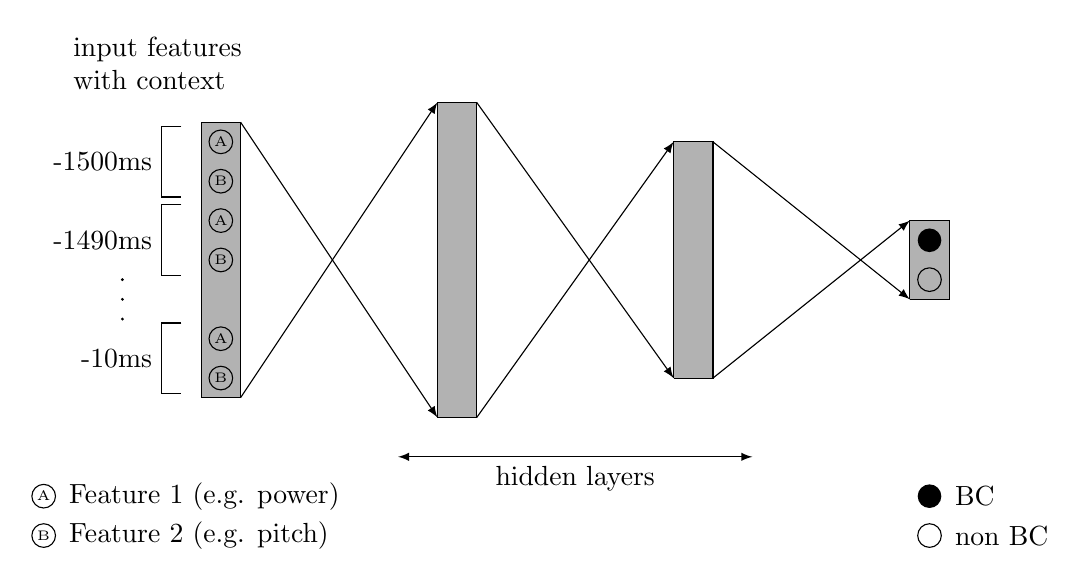
\begin{tikzpicture}[scale=1]
  \def \lha {2}
  \def \lhb {1.5}
  \fill[layer] (0,-1.75) -- (0.5,-1.75) coordinate(l1br) -- (0.5,1.75) coordinate(l1tr) -- (0,1.75) -- (0,-1.75);
  \fill[layer] (3,-\lha) coordinate(l2bl) -- (3.5,-\lha) coordinate(l2br) -- (3.5,\lha) coordinate(l2tr) -- (3,\lha) coordinate(l2tl) -- (3,-\lha);
  \fill[layer] (6,-\lhb) coordinate(l3bl) -- (6.5,-\lhb) coordinate(l3br) -- (6.5,\lhb) coordinate(l3tr) -- (6,\lhb) coordinate(l3tl) -- (6,-\lhb);
  \fill[layer] (9,-0.5) coordinate(o1b) -- (9.5,-0.5) -- (9.5,0.5) --
  (9,0.5) coordinate(o1t) -- (9,-0.5);
  % Input nodes
  \draw[draw=black] (0.25,1.5) circle (0.15) node {\tiny A};
  \draw[draw=black] (0.25,1) circle (0.15) node {\tiny B};
  \draw[draw=black] (0.25,0.5) circle (0.15) node {\tiny A};
  \draw[draw=black] (0.25,0) circle (0.15) node {\tiny B};
  \draw[draw=black] (0.25,-1) circle (0.15) node {\tiny A};
  \draw[draw=black] (0.25,-1.5) circle (0.15) node {\tiny B};
  
  
  \node[left,text width=2.5cm] at (1,2.5) {input features with context};
  \draw (-0.25,1.7) -- (-0.5,1.7) -- (-0.5,0.8) -- (-0.25,0.8) (-0.25,0.7) -- (-0.5,0.7) -- (-0.5,-0.2) -- (-0.25,-0.2) (-0.25,-0.8) -- (-0.5,-0.8) -- (-0.5,-1.7) -- (-0.25,-1.7);
  \draw (-1,-0.25) circle (0.01) ++(0,-0.25) circle (0.01) ++(0,-0.25) circle (0.01);
  \node[left] at (-0.5,1.25) {-1500ms};
  \node[left] at (-0.5,0.25) {-1490ms};
  \node[left] at (-0.5,-1.25) {-10ms};
  
  \draw[draw=black] (-2,-3) circle (0.15) node {\tiny A} +(0.2,0) node [right](power) {Feature 1 (e.g. power)};
  \draw[draw=black] (-2,-3.5) circle (0.15) node {\tiny B} +(0.2,0) node[right](pitch) {Feature 2 (e.g. pitch)};
  
  % Output nodes
  \fill (9.25,0.25) circle (0.15);
  \draw (9.25,-0.25) circle (0.15);
  \fill (9.25,-3) circle (0.15) +(0.2,0) node[right](power) {BC};
  \draw (9.25,-3.5) circle (0.15) +(0.2,0) node[right](pitch) {non BC};
  
  \draw[->] (l1br) -- (l2tl);
  \draw[->] (l1tr) -- (l2bl);
  %\draw (l1br) -- (l2bl);
  %\draw (l1tr) -- (l2tl);
  
  \draw[->] (l2tr) -- (l3bl);
  \draw[->] (l2br) -- (l3tl);
  %\draw (l2tr) -- (l3tl);
  %\draw (l2br) -- (l3bl);
  \draw[->] (l3tr) -- (o1b);
  \draw[->] (l3br) -- (o1t);
  %\node[right](nb) at (9.5,0) {BC};
  \draw[<->] (l2bl) +(-0.5,-0.5) -- ++(4,-0.5);
  \node[below](hL) at (4.75,-2.5) {hidden layers};
  \end{tikzpicture}
  \caption{Feed-forward neural network architecture for backchannel prediction.\label{fig:nn_2h}}
\end{figure}
